\clearpage
\section{Stepper motor}
Stepper motors are electrical motors that can be precisely controlled. They divide a full rotation into a discrete amount of steps, each equally big.

Stepper motors are usually used with a specific circuit to control them, a stepper-motor controller. Stepper-motor controllers allow for microstepping, which further divides a step into smaller pieces. We used 8 micro-steps per step

\begin{figure}[H]
	\centering
	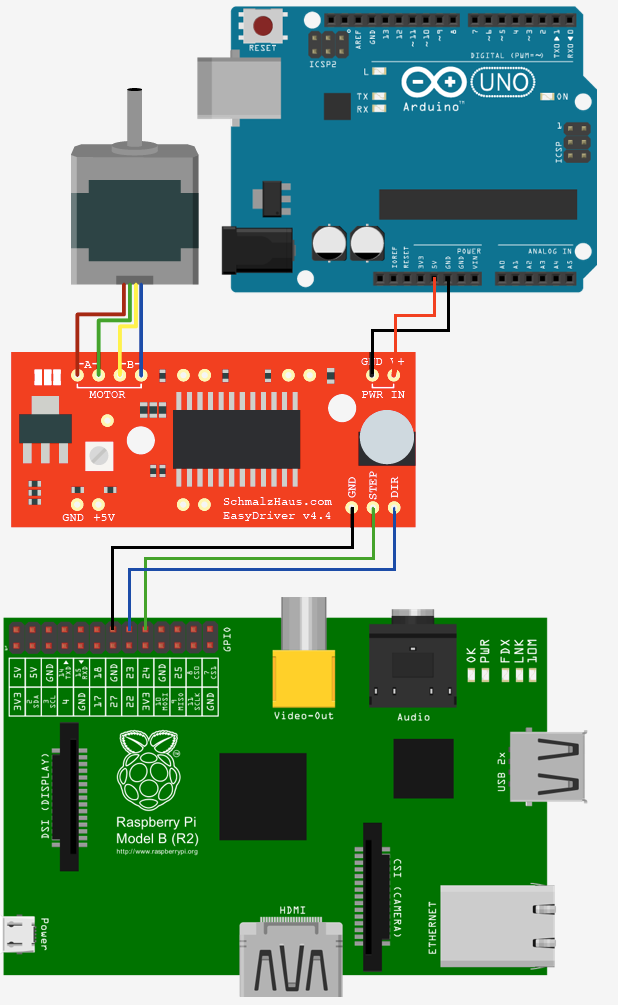
\includegraphics[scale=.5]{images/steppermotor.png}
	\caption{Gustavo will write here}
	\label{fig:steppermotor}
\end{figure}

The stepper motor we used in our project is NEMA-17 Bipolar Stepper Motor. \cite{steppermotor}
The stepper motor controller we used is an EasyDriver.\cite{steppercontroller}

\lstinputlisting[firstline=1, lastline=20, title=Arduino\_Code, language=C++, label=arduinocode1]{../code/arduino_code}

Since the stepper motor we use divides a full cycle into 200 steps, this means that the resolustion is 1.8 degrees per step. At a dictance of 1m, 1.8degrees can resolve a distance of ~3.1cm, and this increases linearly with a larger distance.~\ref{arduinocode1}

$\frac{x}{sin(1.8deg)} = \frac{1m}{sin(89.1deg)}$ \\
$x = \frac{sin(1.8deg)}{sin(89.1deg)}m$ \\
$x = 3.14cm$ \\


